\section{Introduction}
\label{sec:introduction}

% state the learning objective 
The objective of this laboratory assignment is to choose the architecture of the Gain and Output amplifier stages. \par
Firstly, we started this laboratory writing an NGspice script that simulates the the audio amplifier, based on the script given. The transistor models used were the NPN transistor for gain stage and the PNP Transistor for the output stage. We have also measured the output voltage gain in the passband, the lower and upper 3dB cut off frequencies, the bandwidth (which is the difference between the upper and lower cut off frequencies) and the input/output impedances. \par
Then, we have performed incremental modifications to improve the merit, which is calculated using the expression: \par

\begin{equation}
    M = \frac{(VoltageGain)(bandwidth)}{Cost(lower_{Cutoff}freq)}
\end{equation}\par
Where: \par
Cost = cost of resistors + cost of capacitors + cost of transistors \par
Cost of Resistors = 1 monetary unit per kOhm \par
Cost of capacitor = 1 monetary unit per $\mu$ F \par
Cost of transistors = 0.1 monetary units per transistor \par

After that, using octave, we have created a theoretical DC model able to compute de operating point, comparing it to Ngspice’s OP. We have also computed the values of the gain, input and output
impedances separately for the 2 stages, the frequency response $V_{i} / V_{o}$

Firstly, we have created a simple circuit and then we were updating the circuit to improve the figure of merit. The final circuit obtainned is the one shown below in figure (Fig.\ref{fig:circuito}): \par

\begin{figure}[H]
\centering
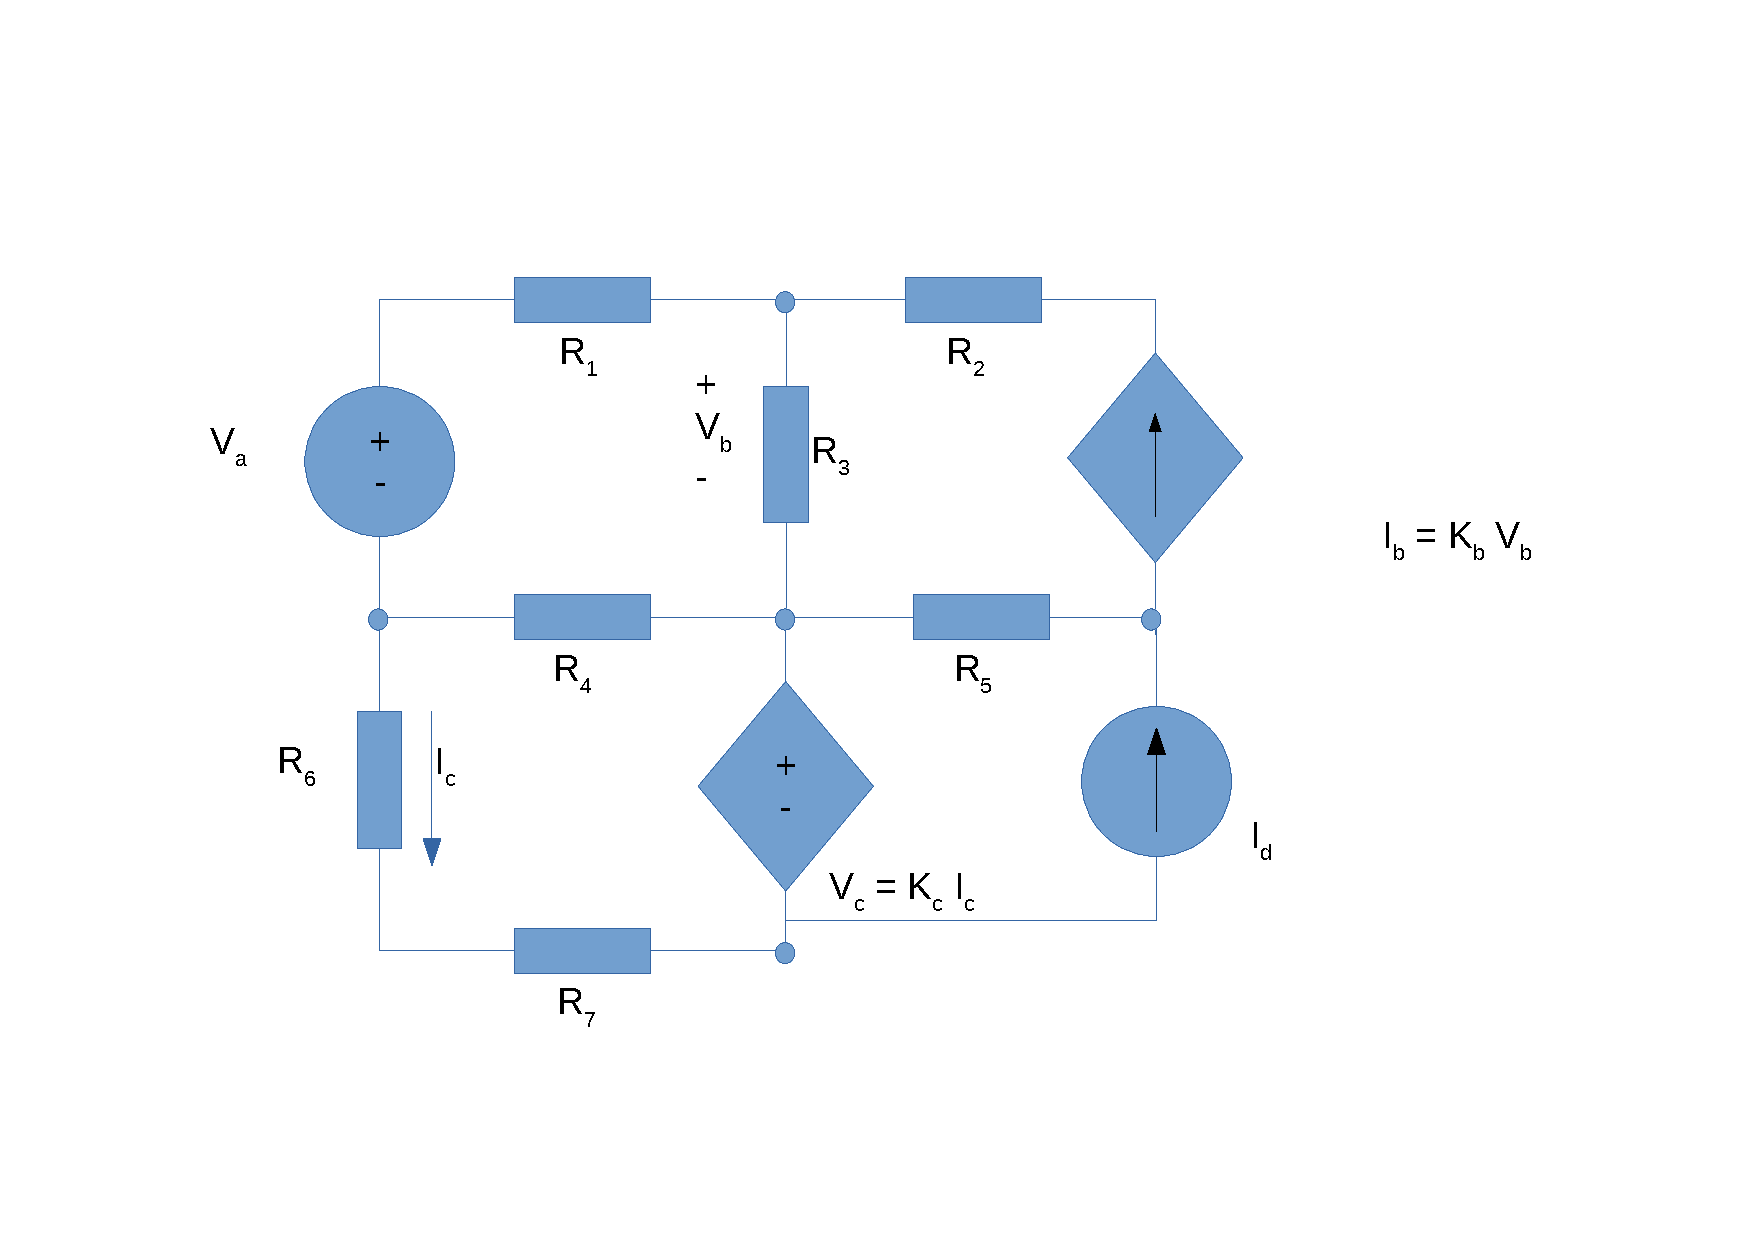
\includegraphics[width=0.9\linewidth]{circuito}
\caption{Final circuit}
\label{fig:circuito}
\end{figure}

The individual costs of the components used: 

\begin{center}
  \begin{tabular}{ | c | c | }
    \hline    
    {\bf Name} & {\bf Value} \\ \hline
    $R$ & 27.3 k$\Omega$ \\ \hline 
    $C$ & 21 $\mu$S \\ \hline
    Transistors & 25 Units \\ 
    \hline
  \end{tabular}
  \captionof{figure}{Costs}
\end{center}



